\documentclass[11pt]{article}   % or 11 pt if you're desperate for space.
\usepackage{amsmath, amssymb, amsthm}
\usepackage{graphicx, microtype, hyperref}
\usepackage{caption}
\usepackage{subcaption}
\usepackage{float}
\usepackage{parskip}
\usepackage{pythonhighlight}
%%%%%%%%%%%%%%%%%%%%%%%%%%%%%
\newcommand{\bkt}[1]{\left( #1 \right)}

%%%%%%%%%%%%%%%%%%%%%%%
% This stuff below sets the page layout. Don't change these.
\addtolength{\topmargin}{-3cm}
\addtolength{\textheight}{5.5cm}
\evensidemargin 14pt
\oddsidemargin 14pt
\textwidth 6.2in
\raggedbottom
\widowpenalty=5000
\clubpenalty=1000
%%%%%%%%%%%%%%%%%%%%%%%

\begin{document}

\title{Using Mathematics with Python}
\author{Student Number 201503311}  % Only give your student number. Marking is kept anonymous.
\date{}   % Leave this blank.

\maketitle

\begin{abstract}

This report will look into the mathematics within Python which allow it to be used to perform various forms of data analysis on a given data set. This is how we're able to make sense of the data we're given and then, for example, use it to provide evidence to a prediction of how the future \textit{"should"} unfold.

\end{abstract}

\section{Introduction}

What is Bayesian analysis in Python? In this article, you will learn about the mathematics for Bayesian statistics that goes on behind the scenes in Python modules. What methods and statistics are used to build up our foundation which we can then start to work with the mathematics to analyse our data to prove, and sometimes disprove, a given hypothesis.

\section{Frequentist and Bayesian Statistics}\label{Frequentist and Bayesian Statistics}

There are two main ways for which we can view probability. One is the \textbf{Frequentist} where the only way a probability is relevant is as the limit of successes in a sequence of trials
$$\hat{p} = \lim_{n\to\infty} \frac{k}{n}$$
Here $k$ is the number of successes and $n$ is the number of trials. But, it wouldn't make sense to link a probability distribution with a parameter, because it doesn't make sense to ask ourselves \textit{"what is the probability distribution on $k$ conditional on the observed value $\hat{p}$?"}. This means that if we were to find the confidence interval we would view the ends as random variables and discuss \textit{"the probability of the confidence interval including the actual parameter"}.

The other is the \textbf{Bayesian} where we see a probability distribution as a way to measure the uncertainty of the world. Thus we can discuss probability distributions of parameters, regardless that the parameter is \textbf{fixed}, because our knowledge of the actual value might be limited. For what we have above, we can flip the probability distribution $p(k\mid \hat{p})$ using Bayes' theorem, to get
\begin{align}\label{Bayes' Theorem}
\overbrace{p(\hat{p}\mid k)}^\text{posterior} = \frac{\overbrace{p(k\mid \hat{p})}^\text{likelihood}}{\underbrace{p(k)}_\text{Evidance}} \overbrace{p(\hat{p})}^\text{prior}
\end{align}
Now there is a slight technicality here, we have to bring in the \textit{prior} to perform our analysis. This represents our \textit{"assumption"} for the value of $p$ before viewing the value $k$. The prior is therefore frowned upon by the frequentist because there is the arguable idea that it brings in subjectivity into the strict manner of probability. But, then again, a prior can be just another assumption made while modelling the situation. Which would then make it just as objective as any of the other assumptions, like the likelihood... But, moving on.

In the Bayesian view, it is not seen as a confidence intervals any more but rather a \textbf{credible interval}. These are a more natural way to interpret the interval. An example would be, \textit{"given a 90\% credible interval, there is a probability of 90\% that the parameter is within the interval"}.

\section{The Prior, Likelihood and Posterior}\label{The Prior, Likelihood and Posterior}

\begin{itemize}
\item The \textbf{prior} is what reflects the information that we know about the value of some parameter before viewing the data $k$. If nothing is known about the parameter then we use a \textbf{flat prior} which doesn't expose much information.
\item The \textbf{likelihood} is our way in introducing the data to the process. It represents how \textit{plausible} the data is while considering the parameters.
\item The \textbf{posterior} is a probability distribution of the parameters in our model. It is what we know about the problem and relates to the prior and the likelihood. If the prior and likelihood are both vague then we'll get a posterior that reflects these vague beliefs. It can be thought of as the updated version of the prior with the given data.
\end{itemize}

The \textbf{evidence} is the probability of getting the data averaged over all possible values. It can be thought of simply as a \textbf{normalising factor} and won't be an issue if we neglect because we're not concerned about the true values of the parameters. Thus, we can rewrite Bayes' theorem as a proportionality (A more general form than our example before)
\begin{align}\label{Bayes' Theorem Proportional}
p(H\mid D) \propto p(D\mid H)p(H)
\end{align}
Where $H$ is the Hypothesis and $D$ is the Data. To gather a true understanding for what each role actually \textit{does}, it'll be beneficial to do a simple example.

\section{Simple Example}\label{Simple Example}

We can consider a very common example that is also very simple; a coin toss. We toss a coin $n$ times and record the number of heads $h$ and tails $t$ we get. Using just this simple data we can deduce answers to possible questions about the problem like \textit{"Is the coin fair?"}. So, to do this, we'll need our data, which is assumed we already have, and a model. 

\subsection{The Model}\label{The Model}

Let's set up an understanding for how the bias can be for this problem. A coin a bias of $1$ will always land on heads. A coin with a bias of $0$ will always land on tails. A coin with a bias of $0.5$ will land on heads and tails evenly. We'll use the parameter $\theta$ for the bias. Then we have the following formula (as seen in \S\ref{The Prior, Likelihood and Posterior} equation (\ref{Bayes' Theorem Proportional}))
\begin{align}\label{Bayes' Theorem Proportional Coin}
p(\theta\mid h) \propto p(h\mid \theta)p(\theta)
\end{align}
Now, we need to choose which prior and likelihood we should use.

\subsubsection{Choosing the Likelihood}\label{Choosing the Likelihood}

Firstly, let's assume that each coin toss is independent of each other. And that only heads
or tails in a possible outcome (no side shots). Then a good distribution for the likelihood
is the \textbf{binomial distribution} because this is a discrete probability distribution for the
number of heads in a sequence of independent 
flips. This is given by:
\begin{align}\label{Binomial Distribution}
p(h\mid\theta) = \frac{n!}{h!(n - h)!}\theta^h(1 - \theta)^{(n-h)}
\end{align}
This gives us the probability (or likelihood) of getting $h$ heads out of $n$ flips, given a fixed bias $\theta$.

\subsubsection{Choosing the Prior}\label{Choosing the Prior}

For this problem it will be wise to use the \textbf{beta distribution}. This distribution is good for our parameter $\theta$ because it is restricted between $0$ and $1$ just like the bias. The first term normalises the distribution so that it will always integrate to $1$. It has two parameters, $\alpha$ and $\beta$, that control the distribution. How it looks is as follows:
\begin{align}\label{Beta Distribution}
p(\theta) = \frac{\Gamma\big(\alpha + \beta\big)}{\Gamma\big(\alpha\big)\Gamma\big(\beta\big)}\theta^{\alpha - 1}\big(1 - \theta\big)^{\beta - 1}
\end{align}
This distribution is something called a \textbf{conjugate prior} to the binomial distribution. This means that we will get a beta distribution as a posterior, since the likelihood is a binomial distribution and the prior is the beta distribution. This makes the posterior capable of being easily controlled mathematically. So that we don't end up with a posterior that we cannot solve. This is an older practice and now, because of computational improvements, this isn't as much of an issue as we could solve numerically with the help of Python. But it'll make things easier for now.

\subsubsection{Getting the Posterior}\label{Getting the Posterior}

This is where we start cooking! (mathematically, of course) Recall equation (\ref{Bayes' Theorem Proportional Coin}) that says the posterior is proportional to the likelihood multiplied by the prior. So, by using equations (\ref{Binomial Distribution}) and (\ref{Beta Distribution}) we get the following:
\begin{align*}
p(\theta\mid h) \propto \bigg(\overbrace{\frac{n!}{h!(n - h)!}\theta^h(1 - \theta)^{(n-h)}}^\text{Likelihood}\bigg)\bigg(\overbrace{\frac{\Gamma\big(\alpha + \beta\big)}{\Gamma\big(\alpha\big)\Gamma\big(\beta\big)}\theta^{\alpha - 1}\big(1 - \theta\big)^{\beta - 1}}^\text{Prior}\bigg)
\end{align*}
To simplify this expression we can drop the terms that do not depend on $\theta$ as we only care about the practical aspect. So we rewrite to find
\begin{align*}
p(\theta\mid h) &\propto \Big(\theta^h(1 - \theta)^{(n-h)}\Big)\Big(\theta^{\alpha - 1}\big(1 - \theta\big)^{\beta - 1}\Big)\\
&\propto \theta^{(\alpha - 1) + h}\big(1 - \theta\big)^{(\beta - 1) + (n - h)}
\end{align*}
There is a relation between this form and the form of the beta distribution.
\begin{align*}
\alpha_\text{posterior} = \alpha_\text{prior} + h,\quad\beta_\text{posterior} = \beta_\text{prior} + (n - h)
\end{align*}
This means that the posterior is the beta distribution.
\begin{align*}
p(\theta\mid h) = \text{Beta}\big(\alpha_\text{prior} + h,\,\beta_\text{prior} + (n - h)\big)
\end{align*}
\subsection{Computing the Posterior}\label{Computing the Posterior}

Using the above analytical expression, we can compute the final result using Python. For example, let's set $\theta = 0.4$, the number of flips $n = 50$ and the number of times we get heads $h = 18$. In a real case, we do not know what the true value of $\theta$ is and for any old coin we would go in assuming that the coin is fair. So we will set our prior to follow this belief. So, we believe that over 50 experiments, we will get $h=25$ and $t=25$. Then our prior is $\text{Beta}(25,25)$. Now, in our real findings, we have that over 50 experiments, we received $h=18$ and $t=32$. Then our posterior is $\text{Beta}(25+18,25+32) = \text{Beta}(43,57)$ (same as above). We can then calculate and plot the results with Python.
\begin{figure}[h]
\centering
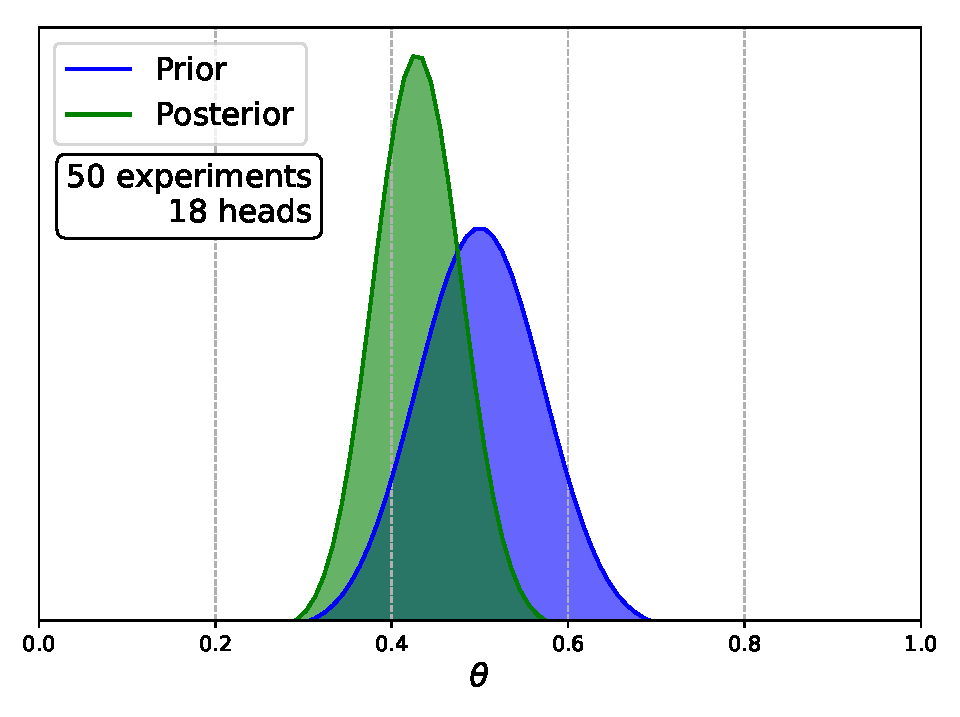
\includegraphics[width = 4in]{Final.pdf}
\caption{Plot of $p(\theta\mid h)$ for set successive experiments.}
\label{figCoinFlipGood}
\end{figure}

The posterior is moving towards the left which would signify that the coin isn't fair and that the bias $\theta < 0.5$. We could approximate the bias as being $\theta \approx 0.43$ so the coin has a sightly higher probability of landing on tails than heads with each flip. It can give us a much better understanding for why the prior is to be chosen with caution if we see the results we get for the posterior when we choose a poor prior.

Let's say we choose the prior to be the belief that over $50$ experiments we will get $40$ heads. Then our prior is Beta$(40,10)$. We shall keep the same data as $50$ flips and $18$ heads. But this poor prior will result in our posterior being Beta$(58,42)$. Obviously, with some understanding and experience of a coin flip, you would never choose a prior like this as it would suggest that you believe the coin has a bias of $\theta = 0.8$. But let us say that maybe a Martian has come whom isn't very familiar with what a coin is and chooses this poor prior. Now we can repeat the process in Python and see the results.
\begin{figure}[H]
\centering
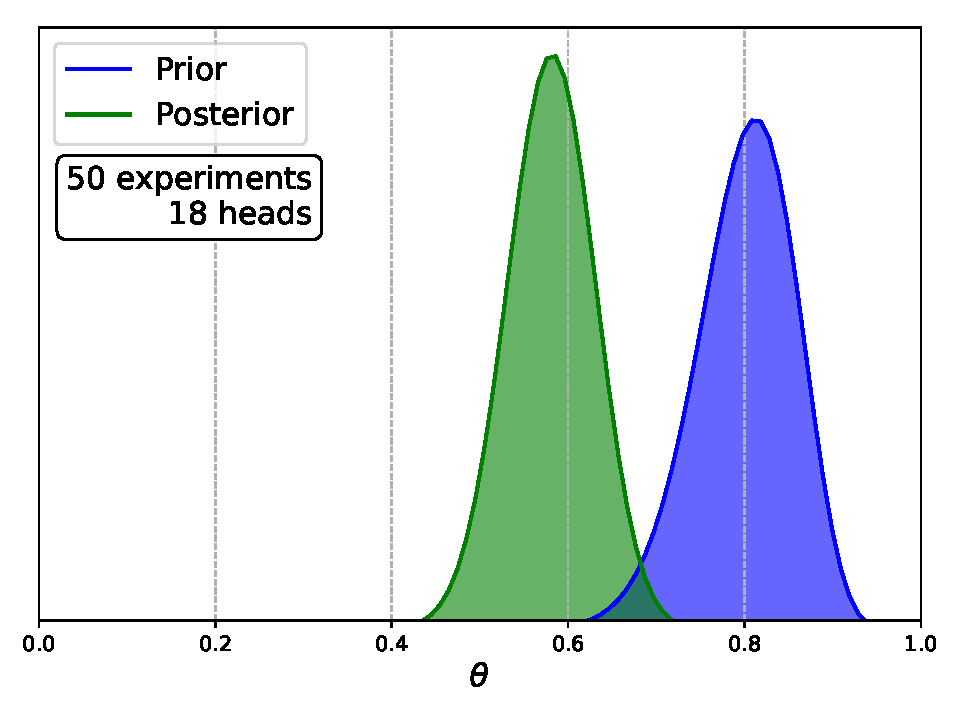
\includegraphics[width = 4in]{BadPrior1.pdf}
\caption{Plot of $p(\theta\mid h)$ with a poor prior.}
\label{figCoinFlipBad1}
\end{figure}
%%%%%%%%%%%%%%%%%%%%%%%%%%%%%%%%%%%%%%%%%%%%%%%%%%%%%%%%%%%%%%%%%%%%%%%%%%%%%%%%%%%%%%%%%%%%%%%%%%
We now see what we suggested before, that the bias would be $40/50 = 0.8$ just as the peak of the prior is very close to that value of $\theta$. The error in the prior then results in error with out posterior. It is giving us the analysis that the coin has a bias of $\theta = 0.6$ which we secretly know isn't right. Although, one thing is that the separation or difference in the distribution is greater than before which could point out that the prior is far off from the true value of $\theta$. So we could then adjust the prior to out \textit{new} belief that the bias of the coin is less than $0.8$.
%%%%%%%%%%%%%%%%%%%%%%%%%%%%%%%%%%%%%%%%%%%%%%%%%%%%%%%%%%%%%%%%%%%%%%%%%%%%%%%%%%%%%%%%%%%%%%%%%%

The posterior is our updated prior given the data above. The black vertical line at $\theta = 0.4$ is there just to illustrate the true value that we have assigned to the bias of the coin. In true practice this would be unknown and we would use the posterior to make a decision on the most plausible value of the bias $\theta$ which is pretty close to at around $\theta \approx 0.38$. This figure gives us an understanding about Bayesian analysis, we see that:
\begin{itemize}
\item The result is a posterior distribution, not a number. It gives us a distribution on the probability with our data.
\item The most plausible value is the peak of the distribution as highlighted before.
\item The spread of the posterior distribution is proportional to the uncertainty of the value for $\theta$. The less spread, the more certain the value.
\item How quickly different posteriors converge to the same distribution depends on the data and the model. After $50$ flips the blue curve is spread away from the posterior.
\item The posterior we get from computing with 150 flips once will be the same as if we computed the posterior 150 times with each one adding one extra observation and using the previous posterior as the new prior.
\end{itemize}

\section{Linear Example}\label{Linear Example}

Here we will use what was discussed in \S\ref{Simple Example} for a more less common example while still being simple in approach. We'll also use more of Python to solve our problem and then discuss the mathematics being used in the background. Our problem is that we are given data and we want to find the original graph. We have the assumption that the original graph is a linear regression and will be of the form: $y = mx + c$. Although there is something extra. This is an exact analytical equation. Our problem will also include a random term called noise. So our problem is to solve the linear equation:
\begin{align*}
y = mx + c + \varepsilon\quad\text{where $m$ is the gradient, $c$ is the intercept and $\varepsilon$ is some noise}
\end{align*}
Now we need to start setting up our model.

\subsection{The Model}\label{The Model2}

We have some data from our mystery linear equation. Now, using this we want to find the equation that produced the data. It's always most useful to plot the data first so that we can make some educated assumptions.
\begin{figure}[h]
\centering
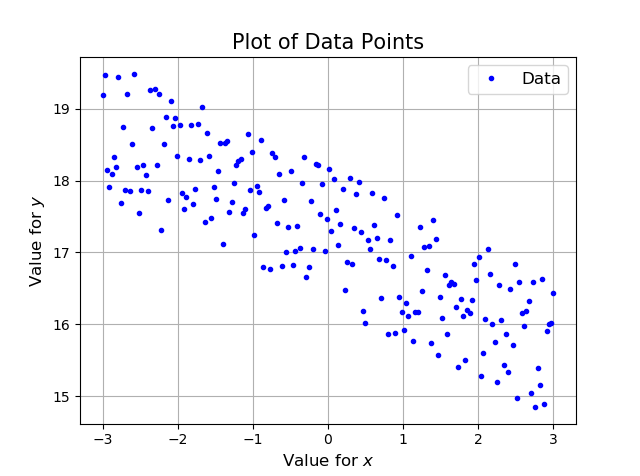
\includegraphics[width = 4in]{Data.png}
\caption{Plot of our given data coordinates}
\label{figLinearData}
\end{figure}

Now we can start to investigate further. Firstly, we can make the assumption that our linear equation will have a negative gradient. There is a general slope in the data from top left to bottom right. Next, we can see  that our data passes through the $y$-axis between $16< y< 19$. So we can assume the the intercept is positive. Combining these two observations will tell us that our equation is of the form: $y = -mx + c$. We will need to conduct Bayesian analysis on our data to conclude what value these two unknowns are, but making these observations are simple yet necessary to build up our prior.

\subsubsection{Choosing the Prior}\label{Choosing the Prior2}

It will be helpful to look into what we will then go on to make as our prior. we can play around with what we have assumed above and plot some values as you will see below. If we try and approximate the centre value at each end of the data cluster then we can think of these as two points. The points will be where our lines cross. Then, if we were to plot a line through these two points, we will plot a linear line that will give us a visual idea of what the real linear equation should look like. Observe:
\begin{figure}[H]
\centering
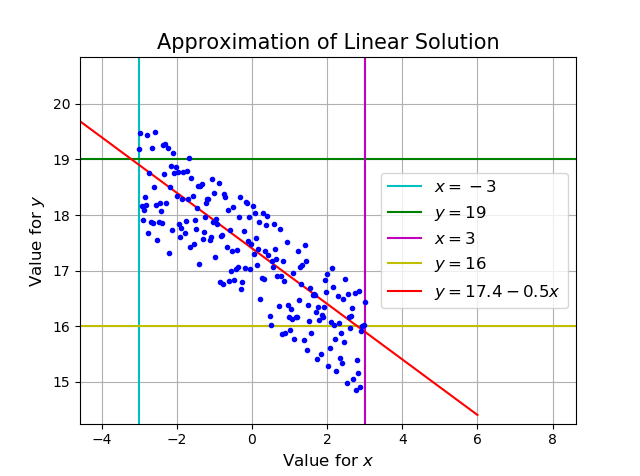
\includegraphics[width = 4in]{Approx.png}
\caption{Plot of approximate values}
\label{figLinearData}
\end{figure}

So now, after looking at our plot, we see that the intercept should be around $c\approx 17.4$ and that the gradient is around $m\approx -0.5$. This is just some clarification mixed with some common sense. We will now go on to decide on our prior for our model but in the back of our minds we will, to some extent, expect to get values like this.

\subsubsection{The Intercept}\label{The Intercept}

We need to think about the best distribution to choose for the parameters we want to find. The intercept, $c$, is a number that will lie between $16<y<19$. So the minimum is $16$ and the maximum is $19$ and we have our $x$ values which is random but it is \textbf{contained} within these values. So I shale choose the prior for the intercept to be a uniform distribution.
\begin{align*}
c \sim U(16, 19)
\end{align*}



\subsubsection{The Gradient}\label{The Gradient}

The gradient, $m$, is \textit{again} a number that will lie between $-1$ and $0$. So, like before, we have a minimum and maximum with our $x$ values between so we will also have our gradient prior as a uniform distribution.
\begin{align*}
m \sim U(-1, 0)
\end{align*}

If we observe what these different graphs look like when compared to the data, it will help to see what has why we chose these values for our uniform priors and how our uniform distribution will work. By choosing these two values, our gradient will \textit{converge} to an estimation of the gradient using Markov chain Monte Carlo (MCMC). It is the same process for the intercept as well. Our two comparisons are seen below:
\begin{figure}[H]
\centering
\begin{subfigure}{0.5\linewidth}
  \centering
  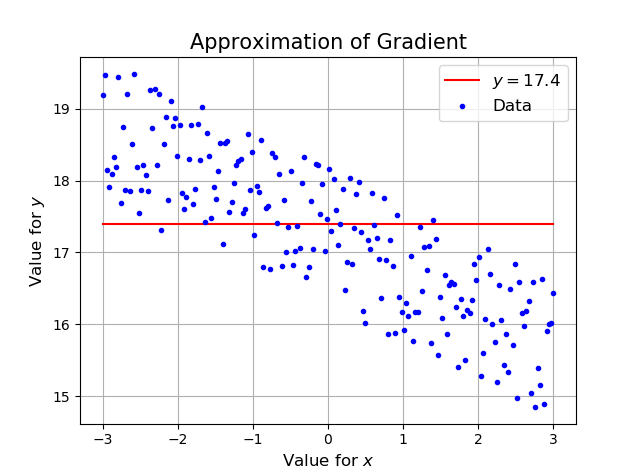
\includegraphics[width = 3in]{gradient0.png}
  \caption{Plot with $m = 0$}
  \label{fig:sub1}
\end{subfigure}%
\begin{subfigure}{0.5\linewidth}
  \centering
  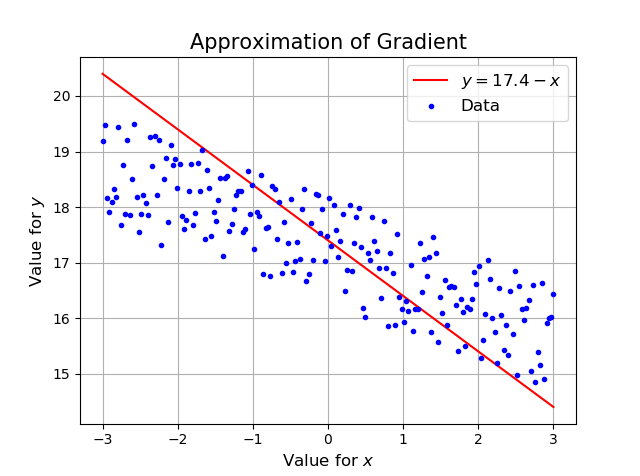
\includegraphics[width = 3in]{gradient1.png}
  \caption{Plot with $m = -1$}
  \label{fig:sub2}
\end{subfigure}
\caption{Comparison of data with different gradient lines}
\label{fig:gradient}
\end{figure}

\subsubsection{Getting the Posterior}\label{Getting the Posterior2}










































\end{document}

The function $f(x) = \cos (x)$ is an \textbf{even} function. It is symmetrical about the \textbf{vertical axis}. We have: $\cos (-x) = \cos (x)$. So:
\begin{align}\label{Intcos}
\int_{-\pi}^{\pi} \cos (\theta)\,d\theta = 0.
\end{align}
We see that the integral is $0$ by the graph $y = \cos (x)$ from $x = -\pi$ to $\pi$. (Figure \ref{figCosineF})

The function $f(x) = \sin (x)$ is an \textbf{odd} function. It is symmetrical about the \textbf{origin}. We have: $\sin (-x) = -\sin (x)$. So:
\begin{align}\label{Intsin}
\int_{-\pi}^{\pi} \sin (\theta)\,d\theta = 0.
\end{align}
Again, it's equal to $0$ by observing the graph $y = \sin (x)$ from $x = -\pi$ to $\pi$. (Figure \ref{figSineF})
\begin{figure}[h]
\centering
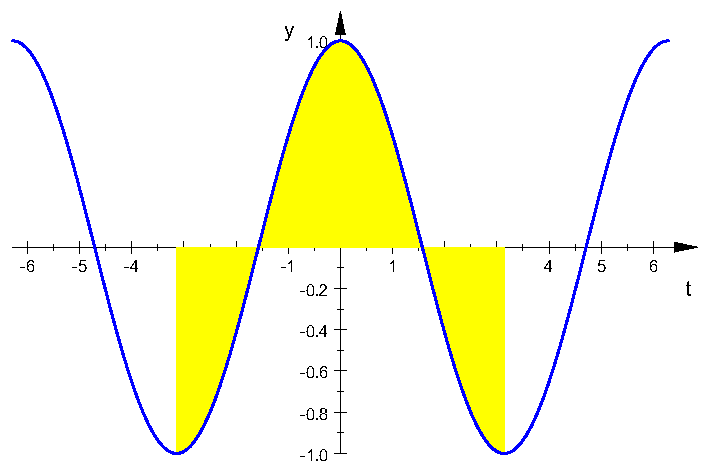
\includegraphics[width = 3in]{CosYellow.pdf}
\caption{The integral of $y = \cos (x)$ from $x = -\pi$ to $x = \pi$.}
\label{figCosineF}
\end{figure}

\begin{figure}[h]
\centering
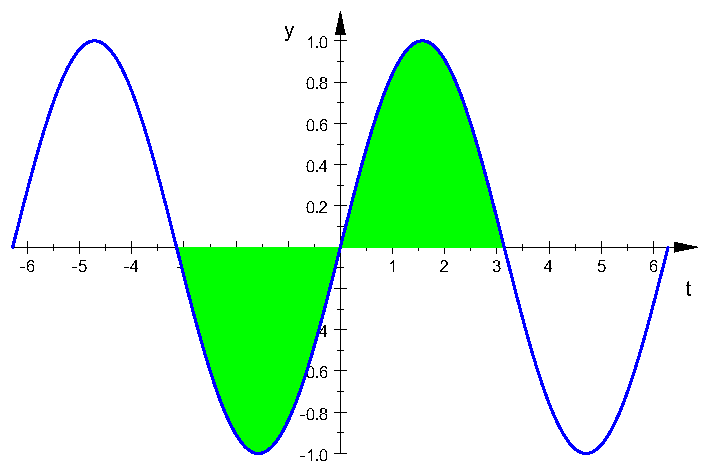
\includegraphics[width = 3in]{SinGreen.pdf}
\caption{The integral of $y = \sin (x)$ from $x = -\pi$ to $x = \pi$.}
\label{figSineF}
\end{figure}

\subsection{Infinite Series}

An infinite series that has a common ratio less than 1 will \textbf{converge}. A numerical example is:
\begin{align*}
1 + \frac{1}{3} + \frac{1}{9} + \frac{1}{27} + \cdots = \frac{3}{2} \quad \text{by the formula} \quad S_\infty = \frac{a_1}{1-r} \quad \text{where $|r| < 1$ and $a_1$ is the first term.}
\end{align*}
We will see functions like the following, which approximates a saw-tooth signal:
\begin{align}
f(x) &= t, \quad \text{if} \quad -\pi \leq t < \pi\\
f(x) &= (t + 2\pi)
\end{align}
The terms in $f(t)$ below create the signal with each term making the approximation more like the exact signal. The series is as follows:
\begin{align}
y = f(t) \approx 2\sin (t) - \sin (2t) + \frac{2}{3}\sin (3t) - \frac{1}{2}\sin (4t) + \frac{2}{5}\sin (5t) + \cdots
\end{align}
\begin{figure}[h]
\centering
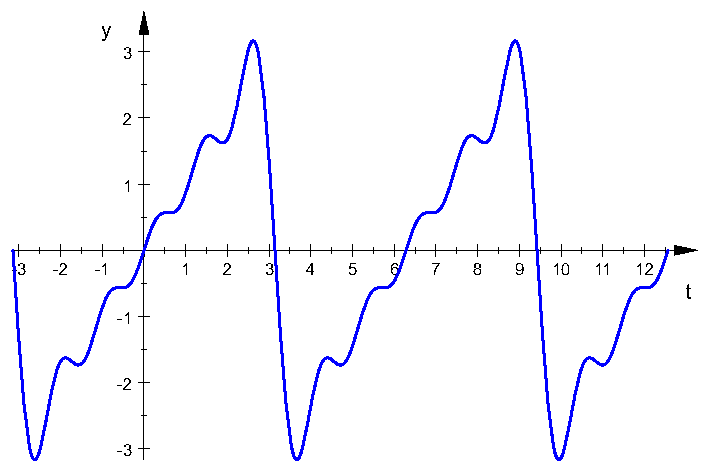
\includegraphics[width = 3in]{SumF.pdf}
\caption{The graph of $y = f(t)$ for $t = -\pi$ to $t = 4\pi$.}
\label{figSumF}
\end{figure}

Note that the Fourier series would \textbf{converge} if we take an infinite number of terms. This was our first goal, but the story goes on.

\subsection{Full Range and Half Range Fourier Series}\label{FRAHRFS}

For the above section you might be thinking "Where do these terms come from?". Well, here's where. Any periodic function of time, denoted $f(t)$, can be resolve into an equivalent infinite summation of sine waves and cosine waves with frequencies that start at 0 and increase in integer multiples of a base frequency $f_0 = \frac{1}{T}$, where $T$ is the period of $f(t)$. The resulting series is the Fourier series. (See \cite{G})

A \textbf{periodic} waveform $f(t)$ of period $T = 2L$ has a Fourier Series given by:

\begin{align}
f(t) &= \frac{a_0}{2} + \sum _{n=1}^{\infty} a_n \cos \bkt{\frac{n \pi t}{L}} + \sum _{n=1}^{\infty} b_n \sin \bkt{\frac{n \pi t}{L}}.\label{FRFS}
\end{align}

\[\text{where $a_n$ and $b_n$ are \textbf{Fourier coefficients}, and $\frac{a_0}{2}$ is the \textbf{mean value}.}\]

\subsection*{Fourier Coefficients}

If $f(t)$ is in the range $-L$ to $L$ (period $T = 2L$), so that the range of integration is $2L$, then the Fourier coefficients are given by:

\begin{align}\label{FRMV}
a_0 &= \frac{1}{L} \int _{-L}^L f(t)\,dt
\end{align}
\begin{align}\label{FCAB}
a_n = \frac{1}{L} \int _{-L}^L f(t) \cos \bkt{\frac{n \pi t}{L}}\,dt, \quad b_n = \frac{1}{L} \int _{-L}^L f(t) \sin \bkt{\frac{n \pi t}{L}}\,dt.
\end{align}

where $n = 1, 2, 3, \ldots$ (All of the above equations see \cite{H})

\subsection*{Even and Odd Functions}

Sometimes, a very pleasant thing happens. The Fourier coefficients $a_0$, $a_n$ or $b_n$ become \textbf{zero} after integration (See \S\ref{SineCosine}).

For an \textbf{even} function $f(t)$, we find that: $b_n =0$. So we only need to find $a_0$ and $a_n$. (see equations \ref{FRMV} and \ref{FCAB})
Thus, an even function has \textbf{cosine} terms:
\begin{align}\label{FREF}
f(t) = \frac{a_0}{2} + \sum _{n=1}^{\infty} a_n \cos \bkt{\frac{n \pi t}{L}}.
\end{align}
For an \textbf{odd} function $f(t)$, we find that: $a_0 = 0$ and $a_n = 0$. The coefficient $b_n$ is given by the equations \ref{FCAB}.
Thus, the Fourier series is:
\begin{align}\label{FROF}
f(t) = \sum _{n=1}^{\infty} b_n \sin \bkt{\frac{n \pi t}{L}}.
\end{align}

An odd function has \textbf{sine} terms. (See \cite{H})

It's similar for \textbf{half range} Fourier series as well. A function can be expanded using half its range of integration, equal to $L$. These are from $0$ to $L$, $-L$ to $0$ and $L$ to $2L$. So, the Fourier series for an \textbf{even} function is equation \ref{FREF}. For an \textbf{odd} function it's equation \ref{FROF}. Though the \textbf{Fourier coefficients}, $a_n$ and $b_n$ (\ref{HFCAB}), and \textbf{mean value}, $a_0$ (\ref{HRMV}), are altered for the new range of integration. (See Appendix for the differences)

\section{Harmonics}

Recall the Fourier series in \S\ref{FRAHRFS} (equation \ref{FRFS}) over the interval $(-\pi ,\pi)$ ($T = 2\pi$), the Fourier series is given by:

\begin{align}\label{FSHA}
f(t) = \frac{a_0}{2} + \sum _{n=1}^{\infty} a_n \cos (n\omega t) + \sum _{n=1}^{\infty} b_n \sin (n\omega t) = \frac{a_0}{2} + \sum _{n=1}^{\infty} \bkt{a_n \cos (n\omega t) + b_n \sin (n\omega t)}
\end{align}
where $\omega = \frac{2\pi}{T} = \frac{\pi}{L}$, $T$ is the period. (See \cite{J}, \cite{G})

The first term is the \textbf{Fundamental}, followed by the \textbf{Second Harmonic} and the \textbf{Third Harmonic}, and so forth.

The Fourier series will be made up of only \textbf{odd harmonics} if $f(t + \pi) = -f(t)$. Here, the Fourier series will be made of all the odd harmonics (odd values of $n$ (equation \ref{OH})). If $f(t + \pi) = f(t)$ then the Fourier series will be made of all the \textbf{even harmonics} (even values of $n$ (equation \ref{EH})). (See \cite{H}) (See Appendix for these forms) 

\section{Fast Fourier Transform}

To go from numbers (MP3) to sound, we need to apply something new. The \textbf{Fourier transform} is a way to represent a function of time as a range of frequencies. The \textbf{Fast Fourier Transform} is a very efficient method to do this. The Fourier transform finds $a_n$ and $b_n$ values to produce a Fourier series, given the base frequency, $f_0 = \frac{1}{T}$ where $T$ is the period of $f(t)$, and the function $f(t)$.

\subsection*{Example}

Say an MP3 has $44100$ samples per second and the length is $1024$ samples, then we find that: $f_0 = \frac{1}{T} = \frac{44100}{1024} = 43.066Hz$. If we process these $1024$ samples with the Fast Fourier Transform, the result will be the coefficients, $a_n$ and $b_n$, for the frequencies. $43.066Hz$, $(2\times43.066) = 86.123Hz$, $(3\times43.066) = 129.20Hz$, etc.

We'll use this to get a series of numbers on an MP3, into a sound. Say we get given:
\[a_0 = 1.6, \quad a_n = \frac{\bkt{-1}^n}{n}, \quad \text{and} \quad b_n = \frac{1}{2n-1}.\]

For the frequencies $43.066Hz$, $86.123Hz$ and $129.20Hz$, we use $\omega = \frac{2\pi}{T}$, (Equation \ref{FSHA}) so:

\[\omega = \frac{44100\times2\pi}{1024} = 270.59.\]

So the Fourier series (equation \ref{FSHA}) would be:

\[f(t) = \frac{1.6}{2} + \sum _{n=1}^{5} \bkt{\frac{\bkt{-1}^n}{n} \cos (270.59nt) + \frac{1}{2n - 1} \sin (270.59nt)}.\]

Computing this summation gives us Figure \ref{figFinalExample}. We've finally managed to rebuild a sound wave! From the data given to us by our hypothetical MP3, it's been made back into sound again which would be done by the MP3 player. This is what we wanted to learn from the start. To produce sound from numbers. This brings us to our conclusion. Things could have been made much more detailed if more space was available because there is still so much to say about the Fourier series. But I'll leave that for another time.

\begin{figure}[H]
\centering
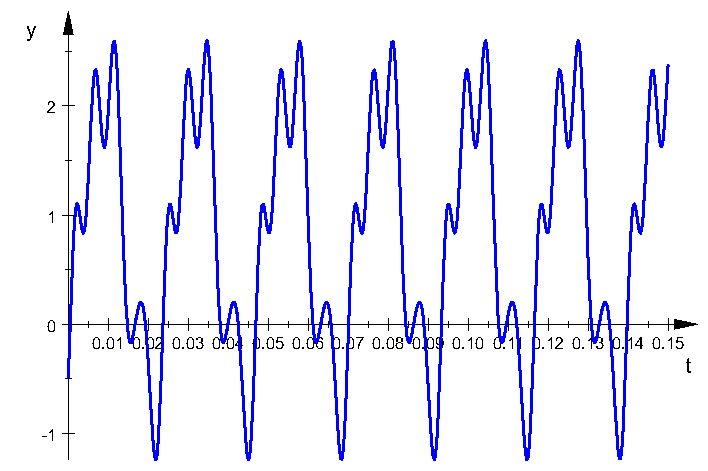
\includegraphics[width = 3in]{FinalExample1.pdf}
\caption{Graph of $f(t)$ for $n = 1$ to $n = 5$.}
\label{figFinalExample}
\end{figure}

\begin{thebibliography}{99}
\bibitem{H} Hardy, G. H. and  Rogosinski, W. W. (2013) \textit{Fourier Series}. Mineola: Dover Publications Inc, 1-4.
\bibitem{J} James, J.F. (2011) Physics and Fourier Transforms. \textit{A student's guide to Fourier transforms: with applications in physics and engineering}. Third Edition. New York: Cambridge university press, 1.2-1.3.
\bibitem{G} Tolstov, G. P. (1976) Trigonometric Fourier Series. \textit{Fourier Series}. Mineola: Dover Publications Inc.
\end{thebibliography}

\section*{Appendix}

\begin{align}\label{HRMV}
a_0 &= \frac{2}{L} \int _{0}^L f(t)\,dt
\end{align}
\begin{align}\label{HFCAB}
a_n = \frac{2}{L} \int _{0}^L f(t) \cos \bkt{\frac{n \pi t}{L}}\,dt, \quad b_n = \frac{2}{L} \int _{0}^L f(t) \sin \bkt{\frac{n \pi t}{L}}\,dt.
\end{align}
\begin{align}\label{OH}
f(t) = \frac{a_0}{2} + \bkt{a_{1} \cos (t) + b_{1} \sin (t)} &+ \bkt{a_{3} \cos (3t) + b_{3} \sin (3t)}\\
&+ \bkt{a_{5} \cos (5t) + b_{5} \sin (5t)} + \cdots\notag
\end{align}
\begin{align}\label{EH}
f(t) = \frac{a_0}{2} + \bkt{a_{2} \cos (2t) + b_{2} \sin (2t)} &+ \bkt{a_{4} \cos (4t) + b_{4} \sin (4t)}\\
&+ \bkt{a_{6} \cos (6t) + b_{6} \sin (6t)} + \cdots\notag
\end{align}

\end{document}